\documentclass[conference,12pt]{IEEEtran}

\usepackage[tight,footnotesize]{subfigure}

\ifCLASSINFOpdf
  \usepackage[pdftex]{graphicx}
  \graphicspath{{./images/}}
\else
\fi

\usepackage[cmex10]{amsmath}


\hyphenation{op-tical net-works semi-conduc-tor}

\begin{document}
	
\title{System Design Project
	\\Group 12 - Robot Unicorn Defenders
	\\Group report 2}

\author{
\IEEEauthorblockN{Jonas Galdikas, Calum Jackson, Daria Kuznetsova, 
Roberto Bezoari,\\ Marc Howarth, Juozas Kaziukenas, Biser Hong, 
Aleksandar Krastev, Behzad Tabibian}
\IEEEauthorblockA{University of Edinburgh}
}
	
\maketitle
\numberwithin{equation}{section}
\IEEEpeerreviewmaketitle

\pagebreak
	
\section{Introduction}
\vspace{-2 mm}
In the third phase of the System Design Project, the main focus of our group was on developing a reliable playing strategy. This involved:
\begin{itemize}
\item Tuning the current robot design to move reliably
\item Improving the existing Vision system to be as accurate as possible
\item Programming simple movement methods that could be used in gameplay strategy
\item Designing and implementing a strategy that would use these methods 
\item Merging aspects of the simulator into robot control, in the form of a GUI
\end{itemize}
\vspace{-2 mm}
\section{Team Organisation}
\vspace{-2 mm}
As of the last milestone, the group svn repository has been migrated from the server provided by the School of Informatics to a dedicated online host. With a dedicated provider such as this, we can be sure of a constant level of service of the grade the we require for a project such as this, where a large number of people must be updating their work regularly, at unpredictable times.  We have also changed our primary method of group communication from a facebook group to a Google group, due to one of the members cancelling their facebook account.
We have been maintaining our website, and all members have been instructed to submit  regular updates about their work, explaining their problems and achievements, to facilitate group integration. This way, everyone should be able to understand the state and structure of the entire project, including parts that they themselves have not been working on. The website has also been used to assign tasks to individual group members with To-Do Lists, so that everyone is contributing to the project at all times. 
\vspace{-2 mm}
\section{Construction}	
\vspace{-2 mm}
At the time of the last report, we were having problems with our robot not moving forwards in a straight line. Over the last two weeks, replacement tyres and a spare motor were procured, as we had established through testing that the combination of a faulty tyre and mismatched motor speeds were at least a large part of the problem. We rebuilt the robot using these new components. It was also decided that to help the robot balance when moving forwards we should move the back stabiliser ball bearing to the front of the robot, and position the driving wheels further back. This way, the majority of the weight would be towards the front end, helping to keep the forwards motion true and minimise wavering. This new design was tested thoroughly on both pitches, and proved to be much more stable, showing reliably straight movement forwards and backwards, and a good turning ability.
We also started experimenting with sensors, thinking that the use of light and touch sensors could improve the movement and shooting accuracy of the robot. A light sensor was positioned behind the kicker, with the aim of detecting when the ball was in prime position for kicking. This required a lot of calibration because the lighting levels in different rooms changed the values of high and low level of light. Marc create a program that calibrated the light levels and output the required parameters automatically. However, the light sensor works by emitting light from a red LED and measuring the percentage of the reflected light from this, and it is possible that this red light might interfere with vision systems, so the plan was put aside. A feature that we decided to retain was the attachment of two touch sensors towards the front end of the robot, for collision detection. This has not yet been implemented fully, but we plan to use the feedback from when the sensors are depressed to create a collision detection system running on the robot client, which would instruct the robot to move backwards, away from whatever obstacle it had encountered, before recalculating the next step in strategy.
\vspace{-2 mm}
\section{Movement and Behaviour}
\vspace{-2 mm}
As movement and behaviour was our main focus for this milestone, a lot of developments were made in this area. An entirely new strategy was developed, with all members of the group contributing in some way. At the low level, this strategy consists of a few simple, trigonometric methods to calculate distances and angles between points, the coordinates of which are received from the vision system. These points can be points on the pitch, the locations of objects on the field, or the location of the goal. Once these have been calculated, the robot can move between the designated points with commands sent to the motors. At a higher level, these methods are utilised by a Strategy class, which models a simple state machine. This works on the basis of a number of ‘if-then-else’ clauses, which describe various situations that might occur on the pitch. These clauses define which movement commands should be executing depending on the state of play. The reasons for implementing such a strategy at this time are several. Firstly, it is simple and easy to understand. This allows everyone to contribute in some way, whether it be code or ideas, even if they are not totally familiar with the intricacies of the various levels  of implementation. Secondly, it allows us to model a large range of situations that may become relevant, including obstacle avoidance, penalties, and choices between attacking and defensive maneuvers.
Another key development in Movement and Behaviour was the integration of some aspects of the simulator’s GUI functionality with the Server code, such as displaying the position of the target points and values of certain variables on screen. The GUI used for simulations (shown in Figure \ref{fig:GUI}) is now the same as the one used for real-life situations, with the ability to select parameters which are as follows:
\begin{itemize}
\item{Goal:} Choose the goal that we are aiming at.
\item{Our Robot:} Determines if our robot is mounted with the blue or yellow plate.
\item{Processor:} Get the location information from either a file, a process (i.e. our vision system) or a simulator.
\item{Strategy:} A list of strategies available to use.
\item{Executor:} Execute the commands on the simulator or through Bluetooth.
\end{itemize}
This simplifies the process of testing our programs, as a single GUI eliminates the need to hardcode certain conditions when testing, and the clear output of variable values has been essential to our debugging process.
\vspace{-2 mm}
\section{Simulator}
\vspace{-2 mm}
Building on the state of the simulator from the last milestone, a collision detection mechanism was added. At first, an external physics library was considered. However, our usage of the simulator is very specific and we designed an algorithm to fit our needs. The different objects handle their own specific collisions: the ball bounces off the walls of the pitch, the robots collide with each other and the walls, and the kicker kicks the ball at the angle of the robot. The current implementation is sufficient for this milestone but the collisions between the robots and the ball are not properly handled. This is set as a goal for the next milestone.
Improving strategy debugging efficiency, we implemented a class that makes drawing to the simulator screen very easy. It abstracts all of the work needed in drawing and provides a better alternative to the previously scattered console printing statements that clogged the code. We can now easily visualize the state of execution of our algorithm, any calculation we doubt or need, and the navigation points outputted by the strategy.
Mouse and keyboard shortcuts provide further functionality like repositioning the objects on the pitch and enabling and disabling the robot in use. The first addition allows us to immediately test the behaviour of the strategy in any imaginable case. The second one allows us to stop the robot from executing commands, thus effectively taking a snapshot of the real-time execution. This way, we can easily examine the current state and the current values of all variables of interest. This is very helpful, as the values of different variables can be changing rapidly while the program is running. Adding real-time parameter tuning capability will decrease testing time, especially in the real robot, and is a goal for the next milestone. 
\section{Vision}
One of the main weaknesses of our program earlier was an unstable Vision subsytem. We could detect objects locations but we could not detect orientaion accurately. One of the main sources of problem was that we always tried to detect orientaion with help of two objects(e.g. balck sport and T. the plate and T). This increased the amount noise caused by detecting each object. 
In this milestone we decided to rely only on one object to detect orientation. This was initially done by finding to points in the shape(i.e. fitting a circle into the object and using its center and center of mass, Figure \ref{fig:centrMass}). This was still not reliable because some times fitted circle was affected by small noises.
Finally we developed a method using \textbf{second order of central moments}. This method proved to be succesfull and become the key to the success of milestone.Mathematical derivatives of calculating orientation is depicted here:
\begin{align}
\mu'_{20} = \mu_{20} / \mu_{00} = M_{20}/M_{00} - \bar{x}^2 \\
\mu'_{02} = \mu_{02} / \mu_{00} = M_{02}/M_{00} - \bar{y}^2 \\
\mu'_{11} = \mu_{11} / \mu_{00} = M_{11}/M_{00} - \bar{x}\bar{y} \\
\Theta = \frac{1}{2} \arctan \left( \frac{2\mu'_{11}}{\mu'_{20} - \mu'_{02}} \right)
\end{align}
\vspace{-2 mm}
\section{Conclusion}
\vspace{-2 mm}
Over the last two weeks, we have strived to fix the communication and organisation failures that led to our poor performance at the last milestone. Everyone has been contributing to the group effort, and the results have been much improved. We achieved all the goals that we set for ourselves for this milestone. For the first friendly match in a week’s time, we hope to have improved the current strategy to be more robust by adding more possible play cases, refining the movement methods and vision data to be more exact still, fully implementing our collision detection sensors, and re-enforcing the body structure of the robot against these collisions, if they happen. We are hopeful that the improved trend in our performance will continue.
\pagebreak
\begin{figure}[htp]
\begin{center}
\leavevmode
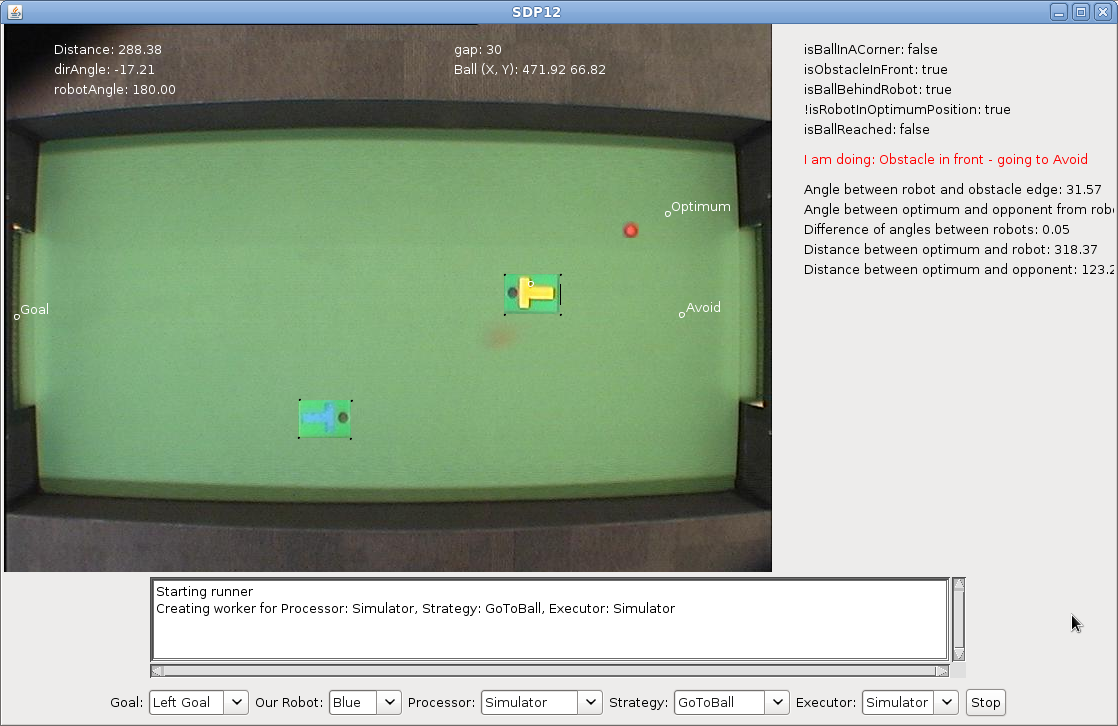
\includegraphics[width=0.4\textwidth] {GUI.png}
\caption{GUI for debugging different algorithms.}
\end{center}
\label{fig:GUI}
\end{figure}

\begin{figure}[htp]
\begin{center}
\leavevmode
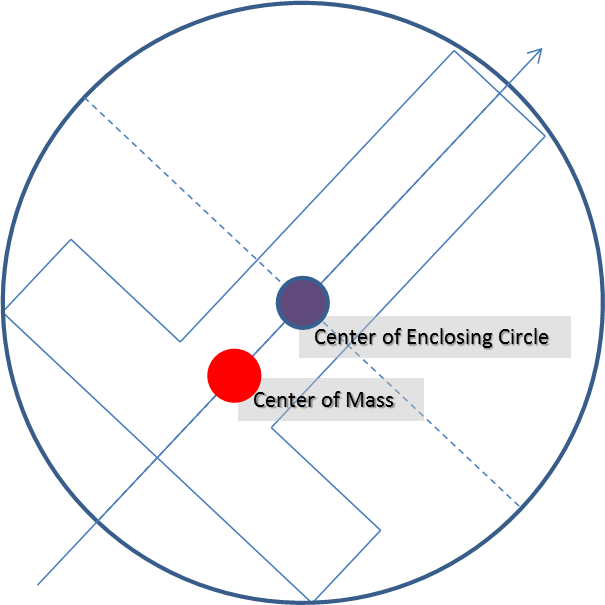
\includegraphics[width=0.3\textwidth] {orientation.png}
\caption{Calculating orientation using center of mass and fitting a circle}
\end{center}
\label{fig:centrMass}
\end{figure}
\end{document}
